\documentclass[11pt]{article}
\usepackage[margin=1in]{geometry}
\usepackage[T1]{fontenc}
\usepackage{lmodern}
\usepackage{booktabs}
\usepackage[table]{xcolor}
\usepackage{array}
\usepackage{longtable}
\usepackage{graphicx}
\usepackage{pgfplots}
\pgfplotsset{compat=1.18}

\title{Supplementary Material for\\
Understanding When Poisson Log-Normal Models Outperform Penalized Poisson Regression for Microbiome Count Data}
\author{Daniel Agyapong, Julien Chiquet, Jane Marks, and Toby Dylan Hocking}
\date{}

\begin{document}
\maketitle

This supplementary document contains the Web Tables and Web Figure referenced in the main manuscript.

\section*{Web Table 1. Count-prediction dataset inventory}
\small
\begin{center}
\begin{tabular}{>{\raggedright\arraybackslash}p{0.24\textwidth}>{\raggedright\arraybackslash}p{0.22\textwidth}>{\raggedright\arraybackslash}p{0.08\textwidth}rrr}
\toprule
Dataset & Human system & Level & $N$ & $D$ & Data sparsity (\%) \\
\midrule
Castro-Nallar 2015 & oral & Genus & 32 & 107 & 60.28 \\
ChngKR 2016 & skin & Genus & 78 & 211 & 80.66 \\
HMP 2012 & nasal & Species & 91 & 222 & 92.72 \\
HMP16S v13 & multi-site 16S & Family & 2909 & 159 & 87.20 \\
American Gut 2 & gut citizen science & OTU & 297 & 138 & 34.48 \\
CosteaPI 2017 & stool enterotypes & Genus & 279 & 179 & 71.73 \\
MehtaRS 2018 & gut longitudinal & Genus & 928 & 183 & 75.72 \\
Diabimmune Karelia & infant gut & Family & 1584 & 55 & 53.36 \\
ShaoY 2019 & infant gut & Genus & 1644 & 244 & 93.01 \\
RubelMA 2020 & pediatric gut & Species & 175 & 373 & 83.85 \\
KarlssonFH 2013 & stool T2D & Genus & 145 & 158 & 71.06 \\
Schubert CDI & stool CDI & Family & 347 & 79 & 79.35 \\
Lozupone HIV & gut HIV & Family & 55 & 62 & 65.75 \\
VilaAV 2018 & gut IBD/IBS & Genus & 355 & 178 & 77.83 \\
Baker NASH/obesity & gut NASH/obesity & Family & 64 & 55 & 56.85 \\
Ross obesity & gut obesity & Genus & 63 & 123 & 67.05 \\
Zeevi obesity & gut glycemic response & Family & 820 & 74 & 74.99 \\
Scheperjans PD & gut Parkinson's & Family & 148 & 40 & 63.04 \\
Littman RA & gut arthritis & Family & 114 & 40 & 67.17 \\
Alkanani T1D & gut T1D & Family & 112 & 27 & 66.34 \\
YuJ 2015 & stool CRC & Genus & 128 & 203 & 72.83 \\
Baxter CRC & stool CRC & Family & 490 & 92 & 71.71 \\
Zeller CRC & stool CRC & Family & 129 & 100 & 58.29 \\
MBQC integrated OTUs & stool benchmark & Family & 18364 & 257 & 89.46 \\
\bottomrule
\end{tabular}
\end{center}
\normalsize

\section*{Web Table 2. Network-inference dataset metadata}
\small
\begin{center}
\begin{tabular}{>{\raggedright\arraybackslash}p{0.18\textwidth}>{\raggedright\arraybackslash}p{0.18\textwidth}>{\raggedright\arraybackslash}p{0.24\textwidth}rrr}
\toprule
Dataset & Human System & Truth type & $N$ & $D$ & Data sparsity (\%) \\
\midrule
OMM12 & defined human gut bacterial community & experimental coculture and dropout interactions & 109 & 12 & 21.25 \\
OMM12 keystone 2023 & defined human gut bacterial community & experimental dropout-derived abundance-ratio effects & 228 & 11 & 31.50 \\
PairInteraX & human gut species panel & experimental pairwise co-culture interaction labels & 169 & 96 & 25.86 \\
Butyrate assembly 2021 & defined human gut community & pair-vs-singleton abundance shifts & 537 & 26 & 66.19 \\
Host fitness 2018 & \textit{Drosophila} gut community & pair-vs-singleton CFU shifts & 1449 & 5 & 54.56 \\
\bottomrule
\end{tabular}
\end{center}
\normalsize

\section*{Web Table 3. Full 28-dataset count-prediction results}
Rows shaded in blue indicate the four strongest PLN-favorable contrasts.
Rows shaded in orange indicate the four strongest GLMNet-favorable contrasts.
\small
\begin{longtable}{p{0.24\textwidth}rrrrrp{0.10\textwidth}}
\toprule
Dataset & $N$ & $D$ & Featureless & GLMNet & PLN & $\Delta$ \\
\midrule
\endfirsthead
\toprule
Dataset & $N$ & $D$ & Featureless & GLMNet & PLN & $\Delta$ \\
\midrule
\endhead
Castro-Nallar 2015 & 32 & 107 & 0.5492 & 0.4857 & 0.3538 & +27.2\% \\
ChngKR 2016 & 78 & 211 & 0.2485 & 0.2139 & 0.1793 & +16.2\% \\
\rowcolor{blue!8} HMP 2012 & 91 & 222 & 0.3386 & 0.3365 & 0.2075 & +38.3\% \\
HMP16S v13 & 2909 & 159 & 0.6972 & 0.3307 & 0.3347 & -1.2\% \\
American Gut 1 & 289 & 127 & 1.8162 & 1.2049 & 1.2761 & -5.9\% \\
American Gut 2 & 294 & 138 & 2.2145 & 1.3108 & 1.1553 & +11.9\% \\
\rowcolor{orange!10} CosteaPI 2017 & 279 & 179 & 0.2515 & 0.1974 & 0.2241 & -13.5\% \\
\rowcolor{orange!10} MehtaRS 2018 & 928 & 183 & 0.2215 & 0.1786 & 0.2225 & -24.6\% \\
\rowcolor{orange!10} Diabimmune Karelia & 1584 & 55 & 1.8574 & 1.1932 & 1.2794 & -7.2\% \\
ShaoY 2019 & 1644 & 244 & 0.2228 & 0.1571 & 0.1647 & -4.8\% \\
RubelMA 2020 & 175 & 373 & 0.1730 & 0.1608 & 0.1473 & +8.4\% \\
KarlssonFH 2013 & 145 & 158 & 0.2607 & 0.2528 & 0.2488 & +1.6\% \\
Schubert CDI & 347 & 79 & 0.9361 & 0.7711 & 0.6905 & +10.5\% \\
\rowcolor{blue!8} Lozupone HIV & 55 & 62 & 1.5514 & 1.3591 & 0.9587 & +29.5\% \\
Gevers 2014 IBD & 285 & 72 & 1.1751 & 0.8396 & 0.7901 & +5.9\% \\
VilaAV 2018 & 355 & 178 & 0.2955 & 0.2587 & 0.2608 & -0.8\% \\
Chan NASH & 54 & 24 & 1.5475 & 1.5787 & 1.2359 & +21.7\% \\
\rowcolor{blue!8} Baker NASH/obesity & 64 & 55 & 1.4737 & 1.3292 & 0.9337 & +29.8\% \\
\rowcolor{blue!8} Ross obesity & 63 & 123 & 1.3015 & 1.2938 & 0.9046 & +30.1\% \\
Zeevi obesity & 820 & 74 & 0.9271 & 0.5570 & 0.5628 & -1.1\% \\
Scheperjans PD & 148 & 40 & 0.8636 & 0.8436 & 0.7713 & +8.6\% \\
Littman RA & 114 & 40 & 1.0220 & 0.9339 & 0.8431 & +9.7\% \\
Alkanani T1D & 112 & 27 & 1.7584 & 1.3291 & 1.0756 & +19.1\% \\
YuJ 2015 & 128 & 203 & 0.2670 & 0.2554 & 0.2515 & +1.5\% \\
Baxter CRC & 490 & 92 & 0.8073 & 0.6112 & 0.5953 & +2.6\% \\
Zeller CRC & 129 & 257 & 1.2164 & 1.0870 & 0.9439 & +13.2\% \\
Zhao CRC & 102 & 78 & 0.7754 & 0.7487 & 0.6205 & +17.1\% \\
\rowcolor{orange!10} MBQC integrated OTUs & 18270 & 235 & 0.6076 & 0.2337 & 0.2996 & -28.2\% \\
\bottomrule
\end{longtable}
\normalsize

\section*{Web Figure 1. Host fitness 2018 network comparison}
\begin{center}

\includegraphics[width=\textwidth]{interaction_network_example_host_fitness_2018_2026-04-01}
\end{center}

\section*{Web Figure 2. Dataset-level winner versus $N/D$ and MAC}
\begin{center}
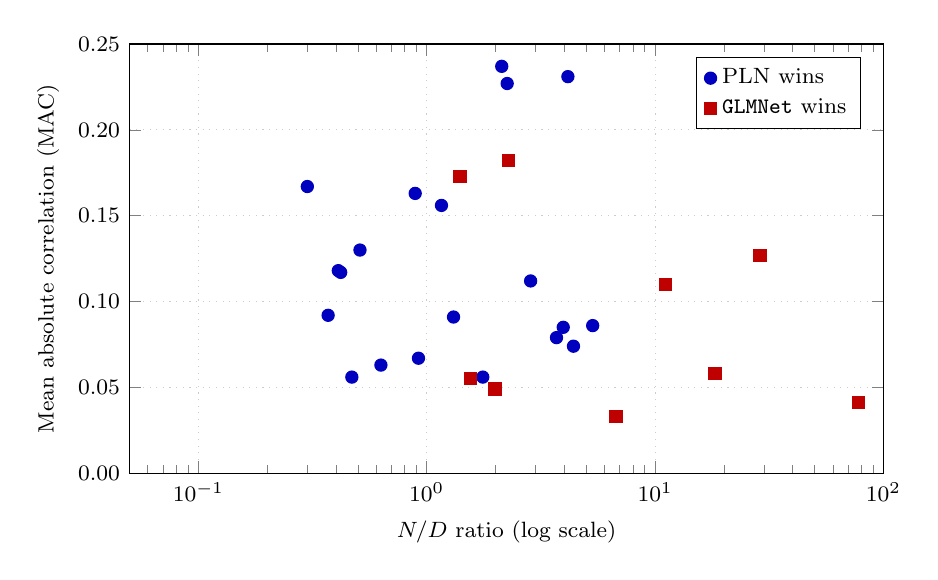
\begin{tikzpicture}
\begin{axis}[
  width=0.92\textwidth,
  height=0.58\textwidth,
  xlabel={$N/D$ ratio (log scale)},
  ylabel={Mean absolute correlation (MAC)},
  xmode=log,
  xmin=0.05, xmax=100,
  ymin=0, ymax=0.25,
  ytick={0, 0.05, 0.10, 0.15, 0.20, 0.25},
  yticklabel style={/pgf/number format/fixed, /pgf/number format/fixed zerofill,
                    /pgf/number format/precision=2, font=\footnotesize},
  ymajorgrids=true,
  xmajorgrids=true,
  grid style={dotted, gray!40},
  tick label style={font=\footnotesize},
  label style={font=\footnotesize},
  legend style={font=\footnotesize, at={(0.97,0.97)}, anchor=north east},
  legend cell align=left,
]
\addplot[only marks, mark=*, mark size=2.2pt, blue!75!black]
  coordinates {
    (0.30,0.167)(0.37,0.092)(0.41,0.118)(0.42,0.117)(0.47,0.056)
    (0.51,0.130)(0.63,0.063)(0.89,0.163)(0.92,0.067)
    (1.16,0.156)(1.31,0.091)(1.76,0.056)(2.13,0.237)(2.25,0.227)
    (2.85,0.112)(3.70,0.079)(3.96,0.085)(4.15,0.231)(4.39,0.074)
    (5.33,0.086)
  };
\addlegendentry{PLN wins}
\addplot[only marks, mark=square*, mark size=2.2pt, red!75!black]
  coordinates {
    (1.40,0.173)(1.56,0.055)(1.99,0.049)(2.28,0.182)
    (6.74,0.033)(11.08,0.110)(18.30,0.058)
    (28.80,0.127)(77.74,0.041)
  };
\addlegendentry{\texttt{GLMNet} wins}
\end{axis}
\end{tikzpicture}
\end{center}

\end{document}
